%----------------------------------------------------------------------------------------
%    PACKAGES AND THEMES
%----------------------------------------------------------------------------------------
\documentclass[aspectratio=169,xcolor=dvipsnames]{beamer}
\makeatletter
\def\input@path{{theme/}}
\makeatother
\usetheme{CleanEasy}
\usepackage[utf8]{inputenc}
\usepackage{polyglossia}
\setmainlanguage{vietnamese}
\usepackage{fontspec}
\setmainfont{Times New Roman}
\usepackage{lmodern}
%\usepackage[T1]{fontenc}
% \usepackage[brazil]{babel}
\usepackage{fix-cm}
\usepackage{amsmath}
\usepackage{mathtools}
\usepackage{listings}
\usepackage{xcolor}
\usepackage{hyperref}
\usepackage{graphicx} % Allows including images
\usepackage{booktabs} % Allows the use of \toprule, \midrule and \bottomrule in tables
\usepackage{tikz}
\usetikzlibrary{positioning, shapes, arrows, calc, decorations.pathreplacing, arrows.meta, backgrounds, patterns, overlay-beamer-styles}
\usepackage{etoolbox}
\usepackage{animate}

%----------------------------------------------------------------------------------------
%    LAYOUT CONFIGURATION
%----------------------------------------------------------------------------------------



% Configure code listings
\lstset{
  basicstyle=\ttfamily\small,
  keywordstyle=\color{blue},
  commentstyle=\color{green!60!black},
  stringstyle=\color{red},
  showstringspaces=false,
  breaklines=true,
  frame=single,
  rulecolor=\color{black!30},
  backgroundcolor=\color{black!5},
  numbers=left,
  numberstyle=\tiny\color{black!70},
  numbersep=5pt
}

%----------------------------------------------------------------------------------------
%    TITLE PAGE
%----------------------------------------------------------------------------------------


%---------------------------------------------


\title[Nice Title]{Fancy and Elaborated Title}

\author[A. Name]{First Author\inst{1} \and  Second Author\inst{2} \and Third Author\inst{3} }

\institute[VFU]{\inst{1}%
  Faculty of Physics\\
  Very Famous University
  \and
  \inst{2}%
  Faculty of Chemistry\\
  Very Famous University 
  \and
  \inst{3}%
  Faculty of Engineering\\
  Another Very Famous University
}


\vspace{-2cm}\date{June 4, 2025}
% Define positions for logos on title page
\titlegraphic{
  \begin{tikzpicture}[remember picture, overlay]
    % 
    \node[anchor=south west, xshift=0.5cm, yshift=0cm] at (current page.south west) {
      
\includegraphics[height=1.3cm]{logos/CleanEasy-logo1.png}
    };

    % 
    \node[anchor=south west, xshift=2.5cm, yshift=0cm] at (current page.south west) {
      
\includegraphics[height=0.9cm]{logos/CleanEasy-logo2.png}
    };
    
    % 
    \node[anchor=north east, xshift=-0.8cm, yshift=-0.3cm] at (current page.north east) {
      
\includegraphics[height=1.1cm]{logos/CleanEasy-logo3.png}
    };
    
    %
    \node[anchor=north east, xshift=-2.8cm, yshift=-0.3cm] at (current page.north east) {
      
\includegraphics[height=1.4cm]{logos/CleanEasy-logo4.png}
    };
  \end{tikzpicture}
}


%----------------------------------------------------------------------------------------


\begin{document}

\begin{frame}[plain]
  \titlepage
\end{frame}

\begin{frame}[plain]{Contents}
  \tableofcontents
\end{frame}

\section{RAN truyền thống và các vấn đề}
\begin{frame}{RAN tổng thể}
  Mạng truy cập vô tuyến (RAN) là một trong những thành phần chính của mạng di động. RAN kết nối thiết bị user equipment (UE) với core network (CN)

  \vspace{0.3cm}
  
  Việc triển khai RAN trong thực tế được gọi là Base Station (BS). Hai đơn vị chính của BS là Radio Unit (RU) và Baseband Unit (BBU). RU chịu trách nhiệm truyền và nhận. Trong khi đó, BBU chịu trách nhiệm quản lý vô tuyến, sử dụng tài nguyên và các hoạt động khác.  Thành phần RAN đã phát triển qua nhiều năm như một giải pháp cho số lượng thuê bao ngày càng tăng và nhu cầu ngày càng cao của người dùng.

\end{frame}

\begin{frame}{D-RAN}
  \begin{columns}[T] % canh top đồng bộ
    % ——————— Cột chữ ———————
    \column{0.7\textwidth}
      Phiên bản đầu tiên của RAN được trang bị một hệ thống tích hợp giữa RU và BBU. BBU thường được lắp đặt trong một căn phòng ngay bên dưới BS. RU có thể được lắp đặt trong phòng hoặc trên đỉnh tháp, cho phép RU hỗ trợ kết nối trong một khu vực rộng lớn. Trong bối cảnh này, RU cũng có thể được gọi là RU từ xa (RRU).
      \begin{itemize}
        \item Khoảng cách giữa RU/RRU và BBU đều ngắn.
        \item Việc triển khai D-RAN rất đơn giản vì nó không yêu cầu giao diện tốc độ cao giữa RU và BBU.
        \item Mạng sẽ dày đặc hơn khi số lượng UE tăng lên và nhiều BS được xây dựng hơn.
        \item Mỗi RAN hoạt động độc lập.
      \end{itemize}

    % ——————— Cột hình ———————
    \column{0.3\textwidth}
      \centering
      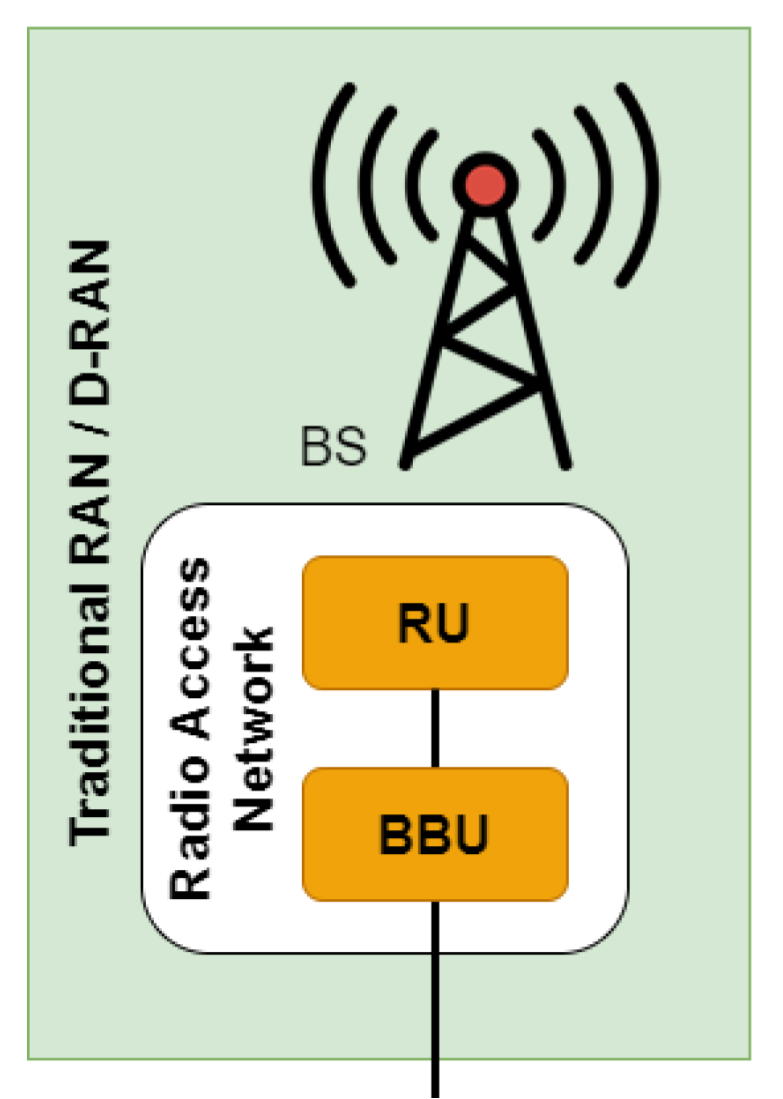
\includegraphics[height=4cm, keepaspectratio]{picture/D-RAN.PNG}
      \\[1ex]
      \small Kiến trúc D-RAN hay RAN truyền thống
  \end{columns}
\end{frame}

\begin{frame}{Vấn đề của D-RAN}
  \begin{columns}[T] % canh top đồng bộ
    % ——————— Cột chữ ———————
    \column{0.4\textwidth}
      \vspace{0.6cm}
      Các nhà khai thác mạng di động (MNO) đã bắt đầu tìm kiếm giải pháp để giảm Chi phí vận hành (OpEx) do chi phí đáng kể cho việc thuê không gian cho BS và hệ thống làm mát cần thiết để vận hành mạng, cuối cùng dẫn đến đề xuất về khuôn khổ C-RAN.

    % ——————— Cột hình ———————
    \column{0.6\textwidth}
      \centering
      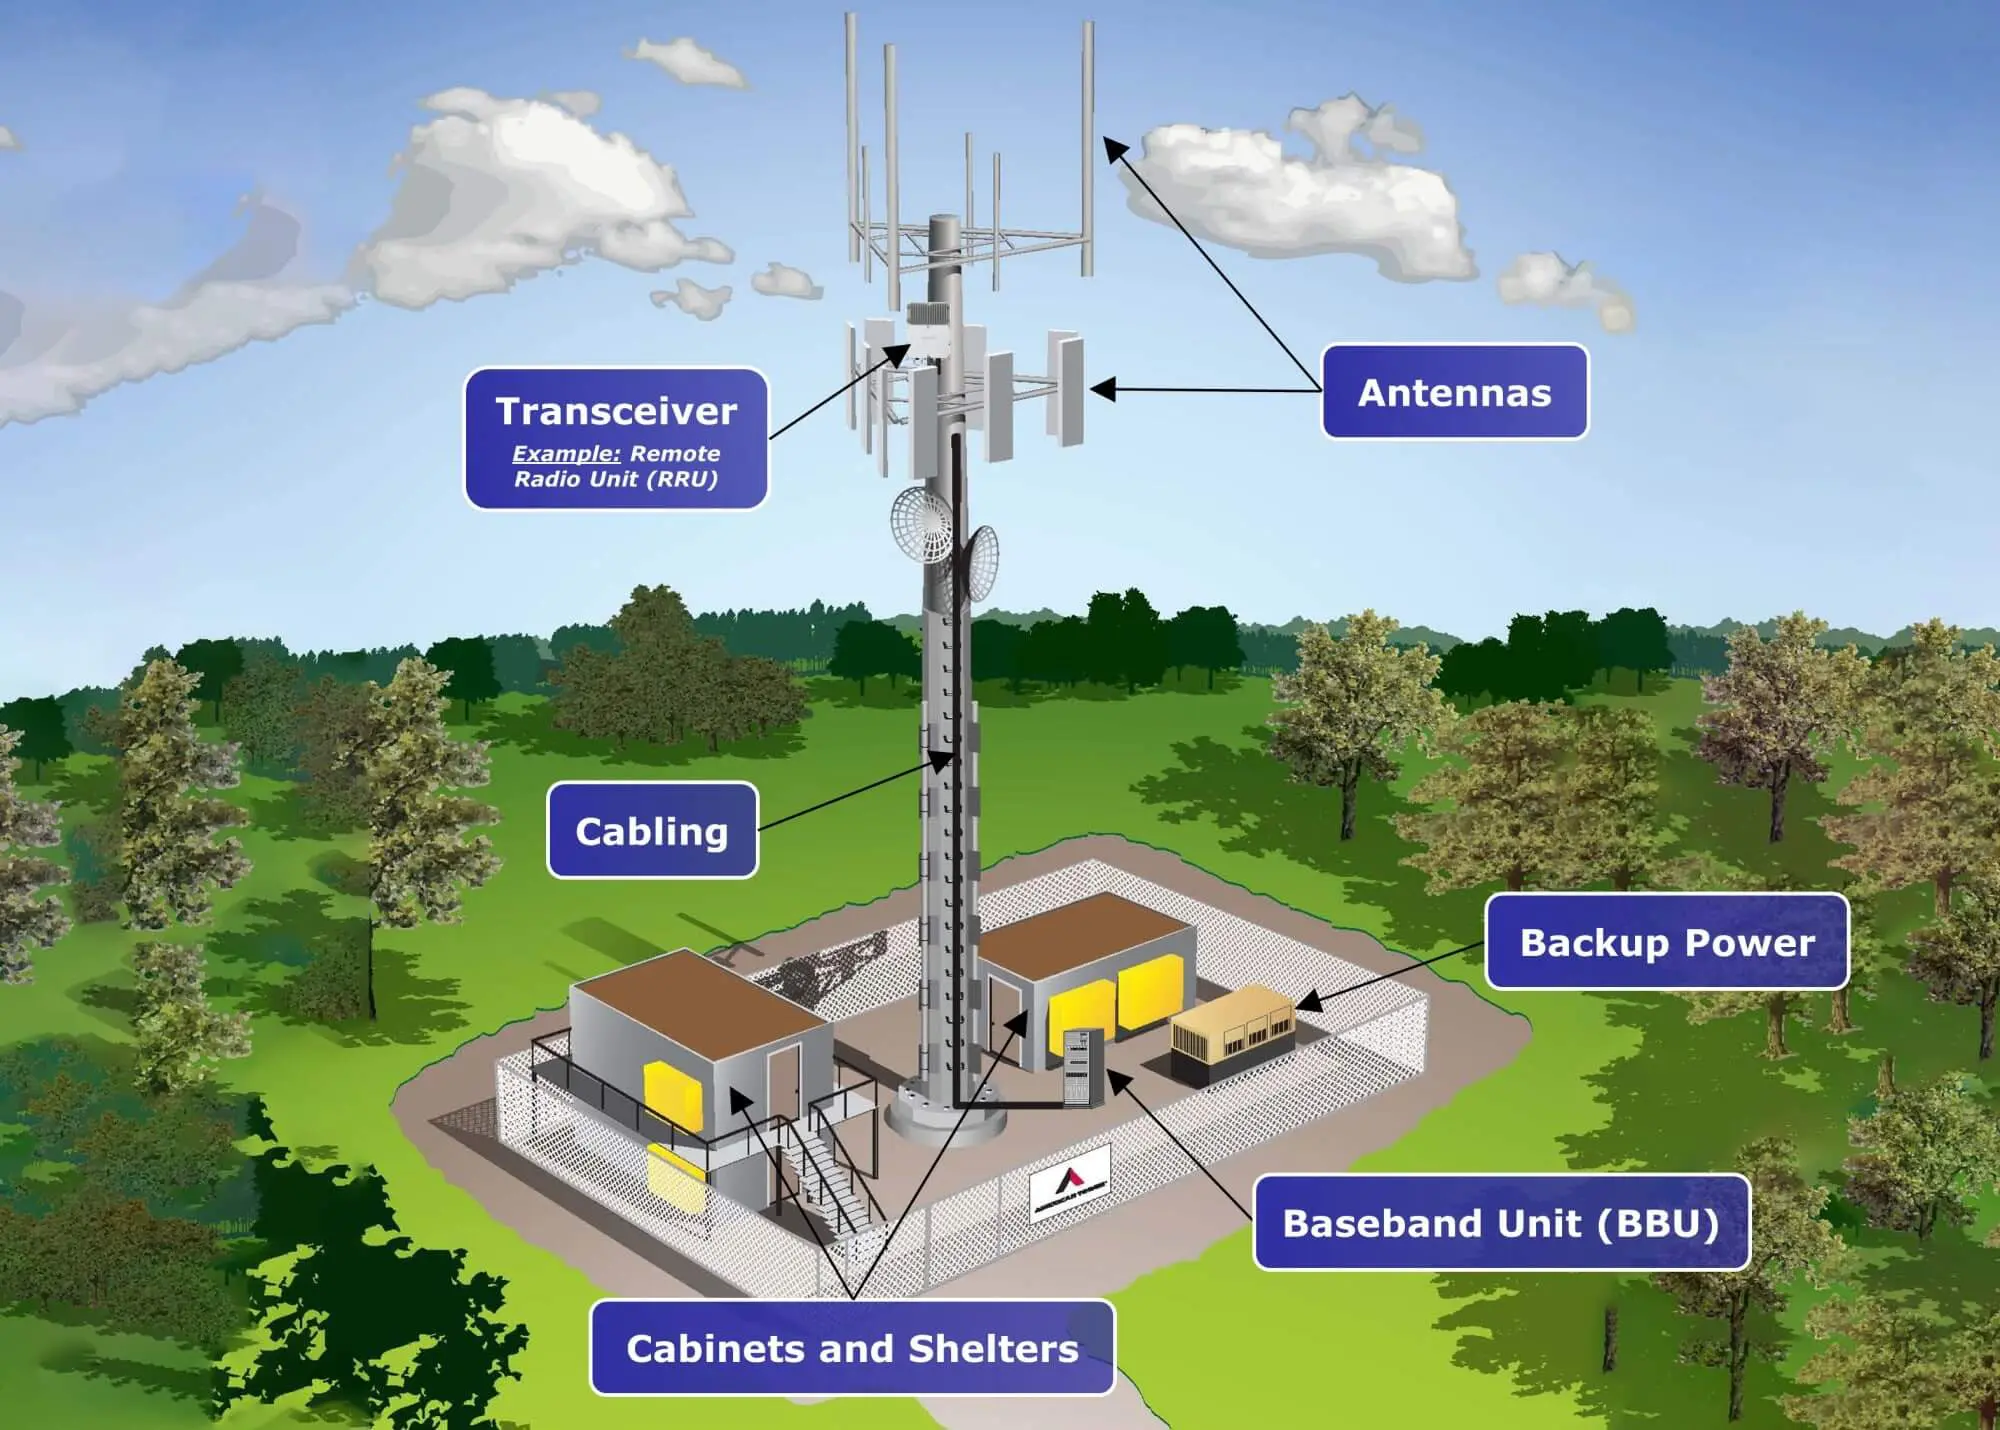
\includegraphics[height=5cm, keepaspectratio]{picture/D-RAN_archi.png}
      \\[1ex]
      \small Mô phỏng 
  \end{columns}
\end{frame}


\begin{frame}{C-RAN}
  \begin{columns}[T] % canh top đồng bộ
    % ——————— Cột chữ ———————
    \column{0.7\textwidth}
      C-RAN có thể hiểu là của Centralized-RAN hoặc Cloud-RAN. Tuy nhiên, cả hai đều có cùng một ý tưởng: nhóm các BBU vào một nhóm
      \begin{itemize}
        \item RAN tập trung được đề xuất để giảm chi phí thuê không gian và mức tiêu thụ điện năng của máy điều hòa không khí của BBU bằng cách nhóm các BBU từ các BS khác nhau vào một vị trí vật lý duy nhất
        \item Fronthaul (FH) là liên kết số hóa giữa các Remote Radio Unit (RRU/RU) đặt tại site và BBU pool 
        \item Mặc dù giảm OpEx tổng thể, RAN tập trung yêu cầu FH phải có băng thông cao và yêu cầu độ trễ thời gian thấp
      \end{itemize}

    % ——————— Cột hình ———————
    \column{0.3\textwidth}
      \centering
      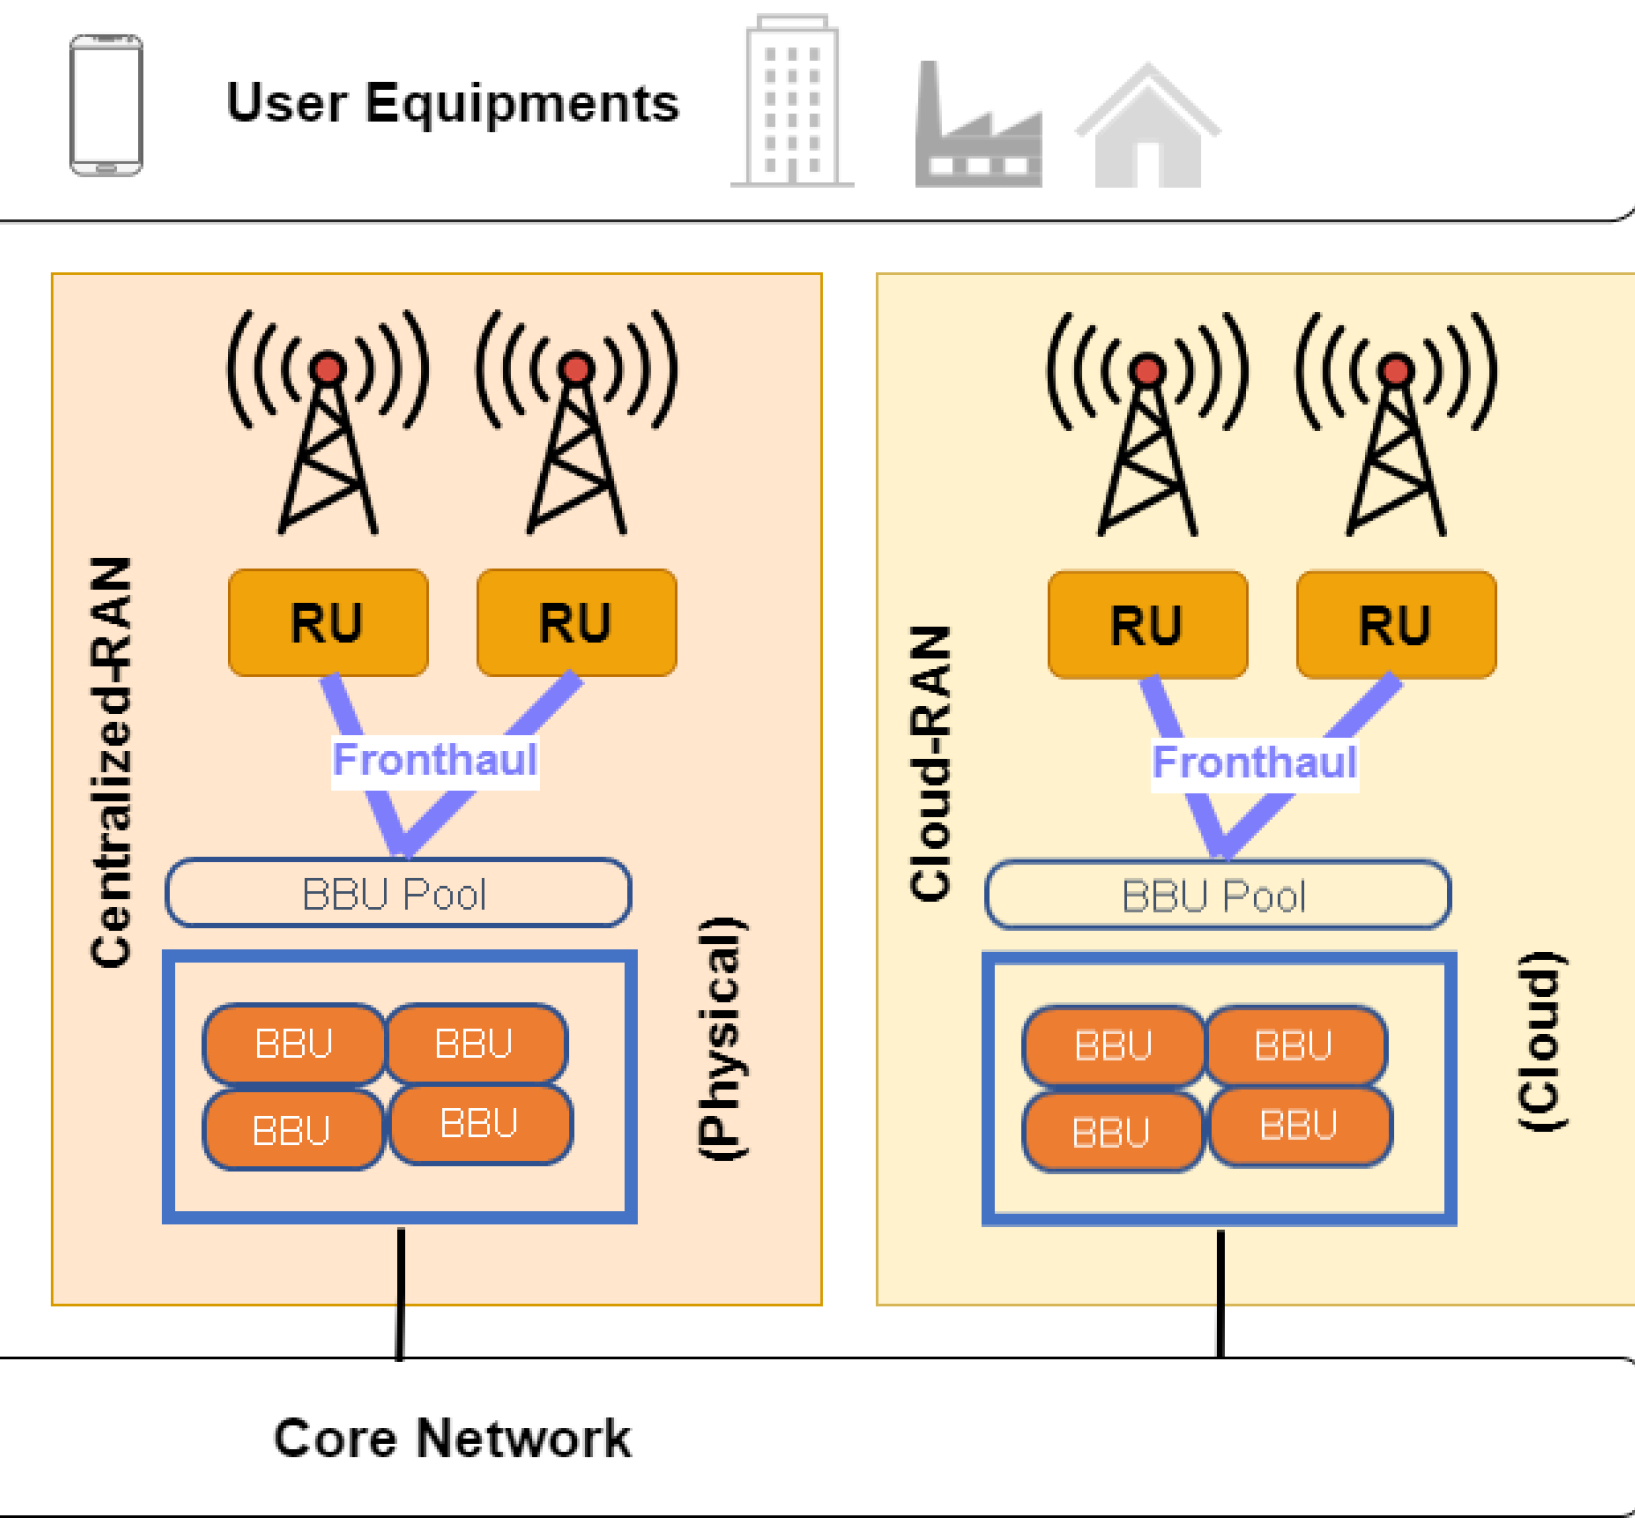
\includegraphics[height=4cm, keepaspectratio]{picture/C-RAN.png}
      \\[1ex]
      \small C-RAN 
  \end{columns}
\end{frame}

\begin{frame}{Khác biệt giữa các biến thể C-RAN}
  \begin{columns}[T] % canh top đồng bộ
    % ——————— Cột chữ ———————
    \column{0.6\textwidth}
      Sự khác biệt cơ bản giữa Centralized RAN và Cloud RAN nằm ở hệ thống cloud. Trong Centralized RAN, các BBU được tập hợp tại một vị trí vật lý còn trong Cloud RAN các BBU từ mỗi BS được tập hợp tại một máy chủ đám mây.
      \begin{itemize}
        \item Cloud RAN giúp dễ dàng thay đổi số lượng BBU theo thời gian.
        \item Cloud cũng tăng khả năng xử lý băng tần cơ sở bằng cách khai thác các bộ xử lý đa năng
        \item Cloud RAN tiếp tục giảm mức tiêu thụ năng lượng, tăng thông lượng mạng, cải thiện khả năng mở rộng mạng, giảm Chi phí vốn (CapEx) và giảm OpEx
      \end{itemize}

    % ——————— Cột hình ———————
    \column{0.4\textwidth}
      \centering
      \vspace{0.3cm}
      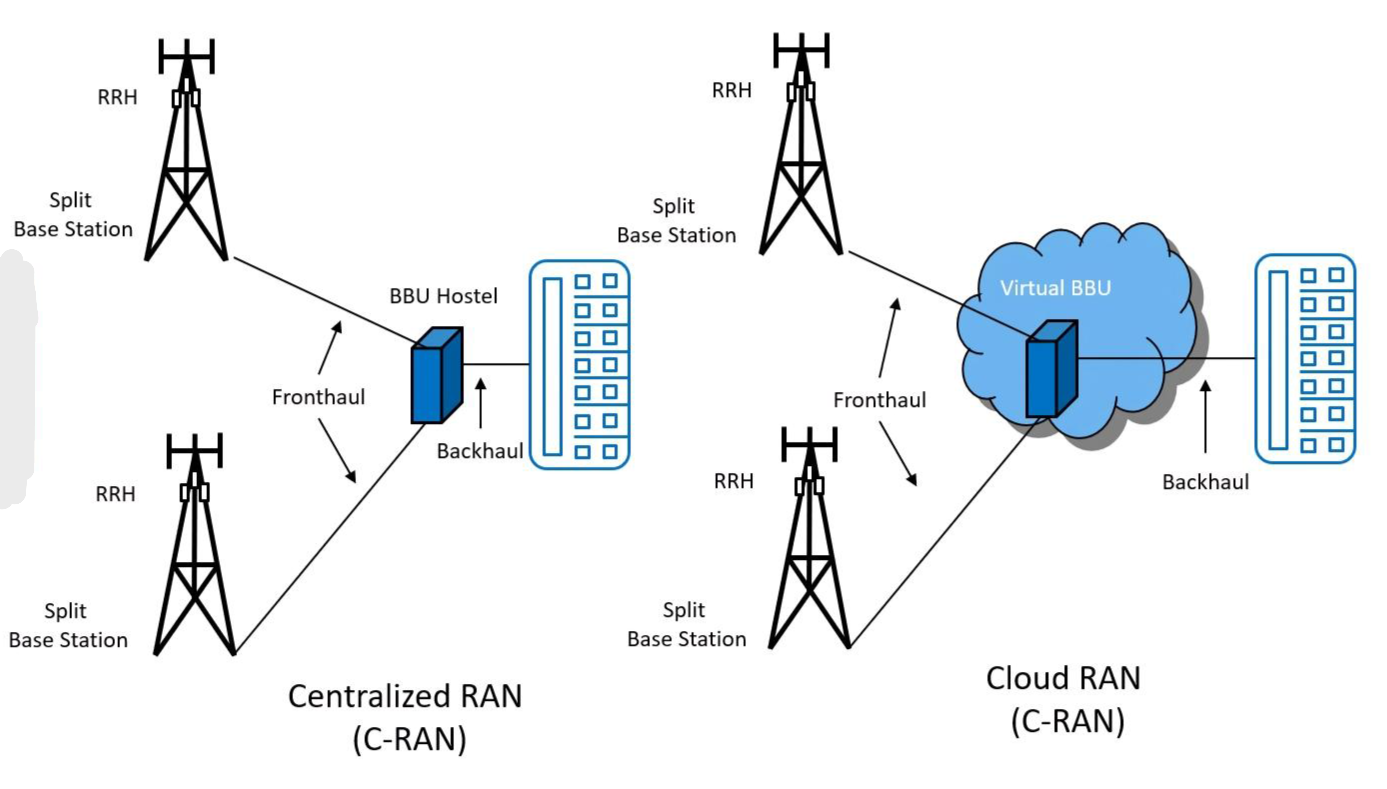
\includegraphics[height=4cm, keepaspectratio]{picture/diff_C-RAN.png}
      \\[1ex]
      \small C-RAN 
  \end{columns}
\end{frame}

\begin{frame}{Vấn đề của C-RAN}
  C-RAN đã được công nhận là một trong những công nghệ tiềm năng nhất để đáp ứng các yêu cầu kỹ thuật 5G của truy cập vô tuyến. 


  \vspace{0.3cm}
  
  
  Tuy nhiên, nó vẫn còn những hạn chế, chẳng hạn như chi phí FH khổng lồ, vấn đề về độ tin cậy, bảo mật và lỗi điểm đơn. Những vấn đề này đã buộc khuôn khổ C-RAN phải chuyển trọng tâm sang các công nghệ điện toán tiên tiến. Một số công nghệ tiên tiến này bao gồm ảo hóa. Ảo hóa là chìa khóa để chuyển đổi từ C-RAN sang vRAN.

\end{frame}

\begin{frame}{vRAN}
  \begin{columns}[T] % canh top đồng bộ
    % ——————— Cột chữ ———————
    \column{0.6\textwidth}
    \vspace{0.4cm}
      Ảo hóa có nghĩa là tạo các phiên bản ảo trên phần cứng vật lý trừu tượng. Trong bối cảnh của vRAN, các phiên bản ảo là tài nguyên mạng. Ảo hóa trong RAN có liên quan chặt chẽ đến các khái niệm như mạng được xác định bằng phần mềm (SDN) và ảo hóa chức năng mạng (NFV). Nói một cách đơn giản, vRAN mang ảo hóa đến với Cloud RAN. Trong máy chủ đám mây, nhiều BBU ảo (vBBU) được triển khai. vBBU có thể được triển khai trên Máy ảo (VM) hoặc vùng chứa.

    % ——————— Cột hình ———————
    \column{0.4\textwidth}
      \centering
      \vspace{0.5cm}
      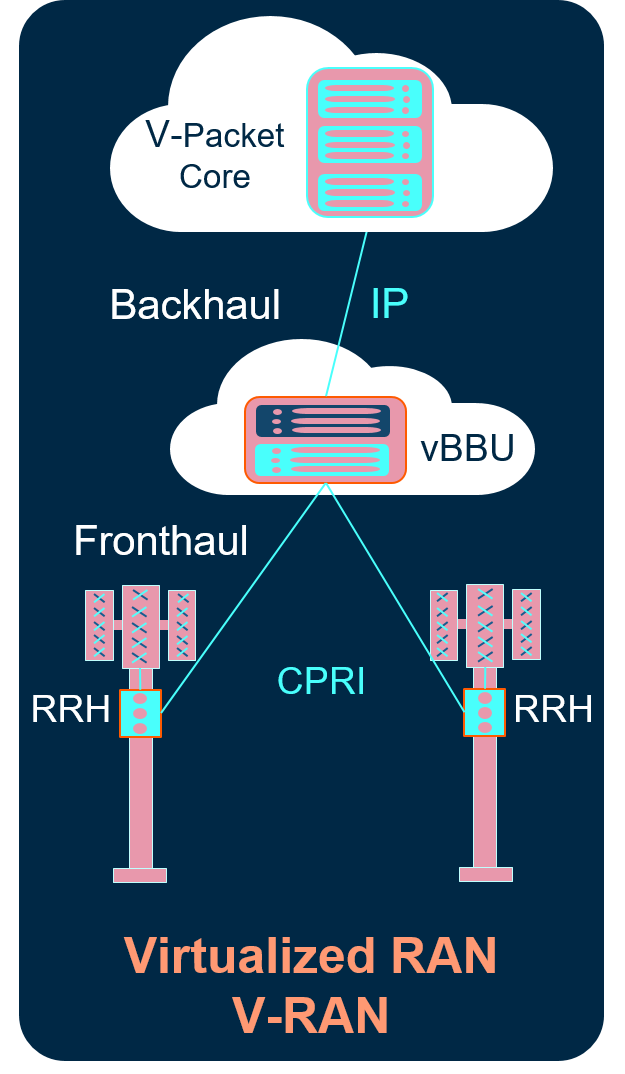
\includegraphics[height=6cm, keepaspectratio]{picture/vRan.png}
      \\[1ex]
      % \small C-RAN 
  \end{columns}
\end{frame}

\begin{frame}{Đột phá của vRAN}
  Hệ thống này cho phép phối hợp và mở rộng tài nguyên trong vRAN. Việc dễ dàng tăng và giảm quy mô tài nguyên mạng dẫn đến : 
  \begin{itemize}
    \item Mức tiêu thụ năng lượng thấp hơn.
    \item Khả năng mở rộng dung lượng động.
    \item Sử dụng hiệu quả tài nguyên mạng.
    \item Cải thiện độ tin cậy của dịch vụ và chất lượng dịch vụ tốt hơn.
  \end{itemize}

  \vspace{0.3cm}

  Khoảng một nửa tài nguyên xử lý dữ liệu cần thiết có thể được giảm khi ảo hóa được áp dụng trên Cloud RAN .

\end{frame}

\begin{frame}{Vấn đề của vRAN}
  Nhìn chung vRAN giảm thiểu chi phí vận hành và đầu tư cho các nhà mạng di động (MNO). 
  
  
  Tuy nhiên 
  \begin{itemize}
    \item vRAN phải xử lý các đặc tính của kênh không dây.
    \item Tài nguyên mạng phải được chia sẻ và phân bổ công bằng và hiệu quả cho các RRU khác nhau.
    \item Cân nhắc các yêu cầu về QoS
  \end{itemize}
  % QoS là  (Quality of Service) là “Chất lượng Dịch vụ” trong mạng viễn thông, dùng để chỉ khả năng mạng đảm bảo các thông số hiệu năng phù hợp với yêu cầu của từng loại ứng dụng.  Cụ thể, QoS thường quản lý và ưu tiên các đặc tính sau:
  % Độ trễ (Latency): Thời gian truyền gói tin từ nguồn đến đích. Các ứng dụng thời gian thực (voice, video call) yêu cầu độ trễ rất thấp.

  % Độ trễ biến thiên (Jitter): Độ không đồng nhất về thời gian đến của các gói tin; jitter cao có thể làm gián đoạn trải nghiệm thoại hoặc video.

  % Tỉ lệ mất gói (Packet Loss): Tỉ lệ gói tin không tới đích; mất gói cao ảnh hưởng xấu đến chất lượng âm thanh, hình ảnh.

  % Thông lượng (Throughput): Lượng dữ liệu truyền thành công trên một đơn vị thời gian; cần cao đối với ứng dụng tải xuống hoặc streaming.

  % Tính ổn định (Reliability): Khả năng duy trì các chỉ số trên liên tục theo thời gian.

  % Trong bối cảnh vRAN, QoS đặc biệt quan trọng vì:

  % Chia sẻ tài nguyên: Nhiều RRU (site) phải dùng chung tài nguyên ảo hóa (CPU, bộ nhớ, đường truyền), nên cần cơ chế điều phối ưu tiên để mỗi luồng dữ liệu (voice, video, IoT…) đạt chỉ số QoS phù hợp.

  % Đa dịch vụ: Mạng 5G/vRAN phải hỗ trợ từ dịch vụ băng thông cao (eMBB) đến dịch vụ độ trễ thấp (URLLC), mỗi loại có ngưỡng QoS khác nhau.

  % Phức tạp điều khiển: Để đảm bảo QoS, hệ thống vRAN phải liên tục giám sát và tự động điều chỉnh phân bổ tài nguyên, dẫn đến độ phức tạp trong thiết kế và vận hành.

  Điều này khiến hệ thống vRAN trở nên phức tạp đáng kể. vRAN cũng vẫn sử dụng các giao diện độc quyền, hạn chế khả năng tương tác và môi trường đa nhà cung cấp. Do đó, việc phụ thuộc vào nhà cung cấp và tình trạng độc quyền khiến giá thiết bị mạng không thể rẻ hơn.
\end{frame}
% \begin{frame}{Introduction}
%   The CleanEasy Beamer theme provides a clean, professional look for academic and business presentations.
  
%   \vspace{0.3cm}
  
%   Key features:
%   \begin{itemize}
%     \item Clean, minimalist design
%     \item Carefully chosen color scheme
%     \item Professional typography
%     \item Flexible block environments
%     \item Customizable footers and section pages
%   \end{itemize}
  
%   \begin{block}{About this template}
%     This presentation serves as both documentation and demonstration, showing the various elements and features available in the CleanEasy theme.
%   \end{block}
% \end{frame}

% \begin{frame}{Block environments}

%   \begin{exampleblock}{Example block}
%     Example blocks can be used to showcase code, examples, or case studies.
%   \end{exampleblock}
  
%   \begin{alertblock}{Alert block}
%     Alert blocks draw attention to critical information, warnings, or caveats.
%   \end{alertblock}
  
%   \begin{theorem}
%     In a right-angled triangle, the square of the hypotenuse equals the sum of squares of the other two sides.
%   \end{theorem}
  
%   \begin{definition}
%     A prime number is a natural number greater than 1 that cannot be formed by multiplying two smaller natural numbers.
%   \end{definition}
% \end{frame}

\section{Methods}
\begin{frame}{Lists and Numbering}
  \begin{columns}
    \begin{column}{0.48\textwidth}
      Bulleted list:
      \begin{itemize}
        \item First level item
        \begin{itemize}
          \item Second level item
          \item Another second level
          \begin{itemize}
            \item Third level item
          \end{itemize}
        \end{itemize}
        \item Another first level item
      \end{itemize}
    \end{column}
    \begin{column}{0.48\textwidth}
      Numbered list:
      \begin{enumerate}
        \item First step
        \begin{enumerate}
          \item Substep one
          \item Substep two
        \end{enumerate}
        \item Second step
        \item Third step
      \end{enumerate}
    \end{column}
  \end{columns}
\end{frame}

\begin{frame}{Tables}
  \begin{table}
    \centering
    \caption{Sample table with booktabs style}
    \begin{tabular}{lcr}
      \toprule
      \textbf{Header 1} & \textbf{Header 2} & \textbf{Header 3} \\
      \midrule
      Row 1, Col 1 & Row 1, Col 2 & 123.45 \\
      Row 2, Col 1 & Row 2, Col 2 & 67.89 \\
      Row 3, Col 1 & Row 3, Col 2 & 456.78 \\
      \bottomrule
    \end{tabular}
  \end{table}
  
  \vspace{0.5cm}
  
  \begin{block}{Table styling}
    The CleanEasy theme works well with the booktabs package for professional-looking tables. 
    Simple color alterations make tables more readable without being distracting.
  \end{block}
\end{frame}

\begin{frame}{Mathematical Equations}
  The CleanEasy theme includes proper mathematical typesetting:
  
  \begin{align}
    E &= mc^2 \\
    F &= G\frac{m_1 m_2}{r^2}
  \end{align}
  
  Maxwell's equations in differential form:
  \begin{align}
    \nabla \cdot \vec{E} &= \frac{\rho}{\varepsilon_0} \\
    \nabla \cdot \vec{B} &= 0 \\
    \nabla \times \vec{E} &= -\frac{\partial \vec{B}}{\partial t} \\
    \nabla \times \vec{B} &= \mu_0 \vec{J} + \mu_0\varepsilon_0\frac{\partial \vec{E}}{\partial t}
  \end{align}
  
  Inline equations like $E = mc^2$ are also properly rendered.
\end{frame}

\begin{frame}[fragile]{Code Listings}
  \begin{lstlisting}[language=Python]
# A simple Python function
def fibonacci(n):
    """Return the nth Fibonacci number"""
    if n <= 0:
        return 0
    elif n == 1:
        return 1
    else:
        a, b = 0, 1
        for _ in range(2, n + 1):
            a, b = b, a + b
        return b
  
# Calculate the 10th Fibonacci number
result = fibonacci(10)
print(f"The 10th Fibonacci number is {result}")
  \end{lstlisting}
\end{frame}

\begin{frame}{Figures and Graphics}
  \begin{columns}
    \begin{column}{0.48\textwidth}
      \centering
      \begin{figure}
        \centering
        % Replace with actual image path
        % \includegraphics[width=\textwidth]{figures/sample_image.png}
        \tikz \fill[blue!30] (0,0) rectangle (3,2);
        \caption{Sample placeholder image}
      \end{figure}
    \end{column}
    \begin{column}{0.48\textwidth}
      \centering
      \begin{figure}          
      \begin{tikzpicture}
        % Simple TikZ diagram
        \draw[thick, ->] (0,0) -- (4,0) node[right] {$x$};
        \draw[thick, ->] (0,0) -- (0,3) node[above] {$y$};
        \draw[blue, thick] (0,0) .. controls (1,3) and (3,1) .. (4,2);
        \node at (2,2.5) {$f(x)$};
      \end{tikzpicture}
      \caption{Simple TikZ diagram}
       \label{fig:enter-label}
      \end{figure}
    \end{column}
  \end{columns}
\end{frame}

\section{Results}
\begin{frame}{Overlays and Animations}
  Beamer supports step-by-step revelations:
  
  \begin{itemize}
    \item<1-> First point appears on slide 1
    \item<2-> Second point appears on slide 2
    \item<3-> Third point appears on slide 3
  \end{itemize}
  
  \pause
  
  This text appears after a pause.
  
  \onslide<4->{
    And this content appears on slide 4.
  }
  
  \begin{block}<5->{Delayed Block}
    This entire block appears only on slide 5.
  \end{block}
\end{frame}

\begin{frame}{Citations and References}
  CleanEasy works well with bibliographies and citations:
  
  \begin{block}{Sample citation}
    % According to Einstein \cite{einstein1905}, space and time are relative.
  \end{block}
  
  \begin{exampleblock}{Bibliography management}
    The theme is compatible with BibTeX, BibLaTeX, and other bibliography management tools.
  \end{exampleblock}
  
  % Sample bibliography entries (not functional without .bib file)
  % \begin{thebibliography}{9}
  % \bibitem{einstein1905}
  %   Albert Einstein.
  %   \emph{On the Electrodynamics of Moving Bodies}.
  %   Annalen der Physik, 1905.
  % \end{thebibliography}
\end{frame}

\begin{frame}{Custom TikZ Graphics}

  \begin{figure}
      \centering
      \begin{tikzpicture}[scale=0.7]
        % Coordinate axes
        \draw[thick, ->] (-3,0) -- (3,0) node[right] {$x$};
        \draw[thick, ->] (0,-3) -- (0,3) node[above] {$y$};
        
        % Unit circle
        \draw[blue!80, thick] (0,0) circle (2);
        
        % Angle and point on circle
        \filldraw[red] (60:2) circle (2pt);
        \draw[red, thick] (0,0) -- (60:2);
        \draw[red, thick, ->] (0.5,0) arc (0:60:0.5);
        \node[red] at (30:0.7) {$\theta$};
        
        % Coordinates
        \draw[dashed] (60:2) -- (60:2 |- 0,0) node[below] {$\cos\theta$};
        \draw[dashed] (60:2) -- (0,0 -| 60:2) node[left] {$\sin\theta$};
      \end{tikzpicture}
      \caption{The unit circle with trigonometric functions}
      \label{fig:exampleTikz}
  \end{figure}
\end{frame}

\section{Conclusions}
\begin{frame}{Theme Customization}
  The CleanEasy theme can be easily customized:
  
  \begin{itemize}
    \item Edit \texttt{beamercolorthemeCleanEasy.sty} to change colors
    \item Modify \texttt{beamerfontthemeCleanEasy.sty} for different fonts
    \item Adjust \texttt{beamerinnerthemeCleanEasy.sty} for layout changes
    \item Update \texttt{configs.tex} for footer and section page customization
  \end{itemize}
  
  \begin{alertblock}{Important Note}
    Always maintain consistent design elements throughout your presentation for a professional look.
  \end{alertblock}
\end{frame}

\begin{frame}{Final Thoughts}
  \begin{block}{Benefits of CleanEasy}
    \begin{itemize}
      \item Professional appearance suitable for academic and business contexts
      \item Careful attention to typography and spacing
      \item High readability with suitable contrast ratios
      \item Flexible design that works with different content types
    \end{itemize}
  \end{block}
  
  \vspace{0.5cm}
  
  \begin{center}
    \large{The CleanEasy theme is designed to let your content shine without distractions}
  \end{center}
\end{frame}

\begin{frame}[plain]
  \centering
  \Huge \textbf{Thank you!}
  
  \vspace{1cm}
  \normalsize
  \href{mailto:your@email.com}{your@email.com}
  
  \vspace{0.5cm}
  \small
  \texttt{https://someurl.com}
\end{frame}

% Sample bibliography (not shown in presentation, just for reference)
\begin{frame}{References}
  \begin{thebibliography}{9}
    \bibitem{einstein1905}
      Albert Einstein.
      \emph{On the Electrodynamics of Moving Bodies}.
      Annalen der Physik, 1905.
    
    \bibitem{beamer}
      Till Tantau.
      \emph{The Beamer Class}.
      \url{https://ctan.org/pkg/beamer}
  \end{thebibliography}
\end{frame}

% \begin{frame}{References}
%   \bibliography{reference.bib}
%   \bibliographystyle{apalike}
% \end{frame}

\end{document}